\documentclass[a4paper,zihao=5,UTF8]{ctexart}
\usepackage[top=2.3cm,bottom=2cm,left=1.7cm,right=1.7cm]{geometry} 
\usepackage{amsmath, amssymb}
\usepackage{color}
\usepackage{hyperref} 
\usepackage{pythonhighlight}
\usepackage{listings}
\usepackage{mathrsfs} 
\usepackage{booktabs}
\usepackage{amsthm}
\usepackage{longtable} 
\usepackage{graphicx}
\usepackage{subfigure}
\usepackage{caption}
\usepackage{fontspec}
\usepackage{titlesec}
\usepackage{fancyhdr}
\usepackage{latexsym}
\usepackage{subfigure}
\usepackage{braket}
\usepackage{cite}
\usepackage[version=4]{mhchem}

\CTEXsetup[format={\Large\bfseries}]{section}
\def\d{\mathrm{d}}
\def\e{\mathrm{e}}
\def\i{\mathrm{i}}
\def\dps{\displaystyle}
\newcommand{\mr}[1]{\mathrm{#1}}
\newcommand{\mb}[1]{\mathbf{#1}}
\newcommand{\dv}[2]{\frac{\d{#1}}{\d{#2}}}
\newcommand{\pdv}[2]{\frac{\partial{#1}}{\partial{#2}}}
\def\degree{$^{\circ}$}
\def\celsius{^{\circ}\mr{C}}
\title{\textbf{实验三 \ce{KH_2PO_4}(KDP)单晶及\ce{Au}纳米棒的合成和表征\cite{inorganic_chemistry_1}}}
\author{王崇斌\;1800011716}
\makeatletter
\makeatother
\begin{document}
	\pagestyle{fancy}
	\pagestyle{fancy}
    \lhead{无机化学实验}
	\chead{}
	\rhead{\today}
	\maketitle
    \thispagestyle{fancy}
	\section{实验原理}
    \subsection{KDP单晶结构与降温法培养单晶}
    磷酸二氢钾(KDP)晶体是一种优良的非线性光学晶体,在工业中有广泛的用途,因此培养
    其单晶很有实际意义。本实验中通过培养KDP晶体、观察晶体生长过程来了解晶体生长的
    基本规律。KDP属于四方晶系,晶胞参数a = b = 7.4528 nm,c = 6.9717 nm,Z = 4。
    其单晶理想外形为四方柱和两个四方锥的聚合体,四方柱的表面为[100]面,四方锥扣在
    四方柱的上下底面,其表面为[110]面,它的晶体结构和理想外形如图
    \ref{KDP crystal structure} \ref{KDP crystal grow}所示。
    由于晶体生长过程中的各种因素影响,实际得到的KDP单晶常偏离理想外形。
    \begin{figure}[htbp]
        \centering 
        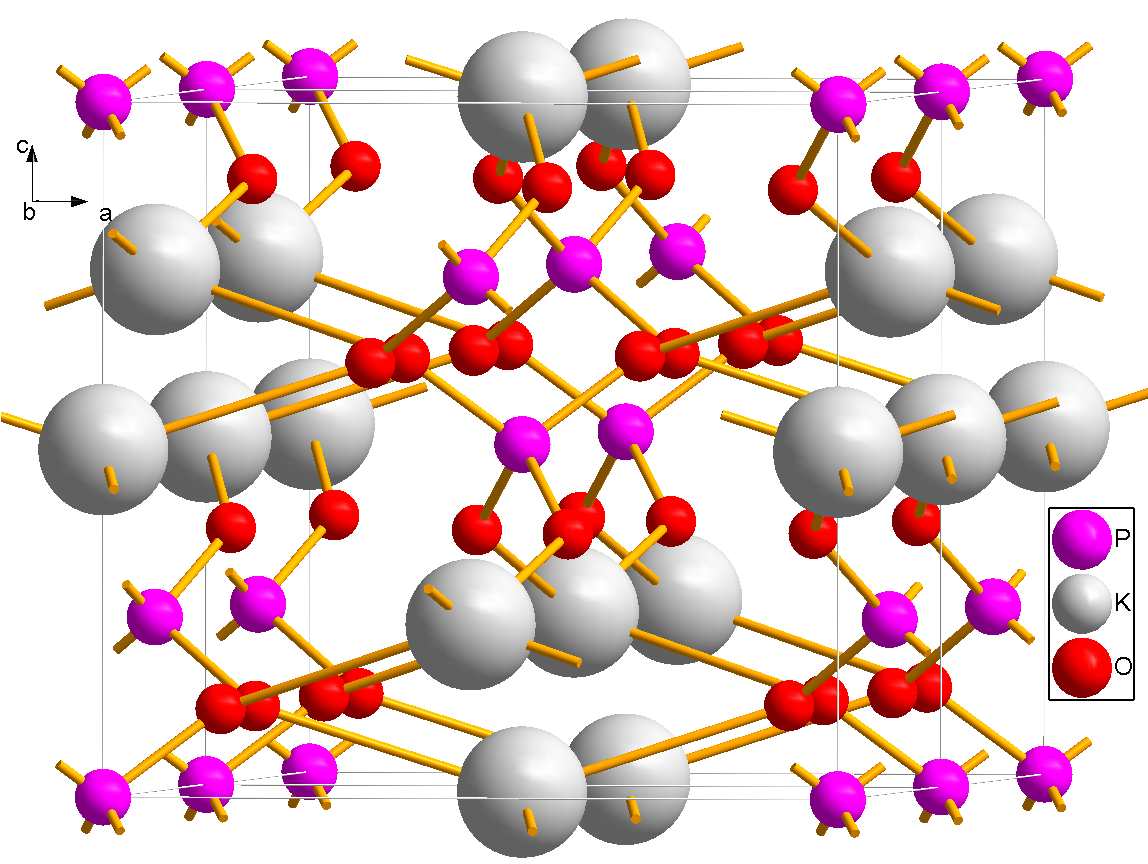
\includegraphics[scale=0.15]{TetragonalKH2PO4structure.png}
        \caption{KDP的晶体结构(图中展示了两个晶胞)}
        \label{KDP crystal structure}
    \end{figure}
    \begin{figure}[htbp]
        \centering 
        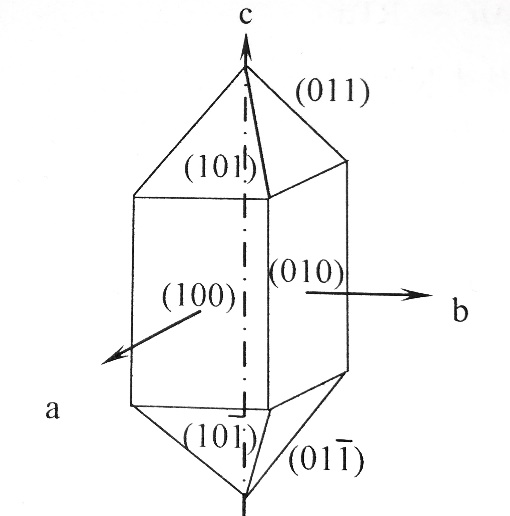
\includegraphics[scale=0.8]{KDPgrow.png}
        \caption{KDP的生长习性}
        \label{KDP crystal grow}
    \end{figure}
    \par 
    降温法是一种常用的培养单晶的方法,其利用大多数溶质溶解度随温度下降这一特性来生长晶体。
    当溶液的过饱和度不太大时,晶体生长的驱动力(严格来说应该用化学势来描述)正比于溶液的过饱和度,
    只有过饱和溶液中可以析出晶体。过饱和溶液可根据溶质析出的特点进一步分为亚稳状态、不稳定状态,
    处于亚稳状态的溶液只会在溶液中含有晶核或者机械杂质时,在这些物质表面析出晶体,处于
    不稳定状态的溶液会自发快速的析出大量晶体。因此,降温法培养晶体的关键是温度的降低速率
    一定要小,保持溶液处于略微过饱和但是处在亚稳状态的情况下结晶,同时要保证溶液中
    机械杂质尽可能少,防止晶体在其上析出。
    \subsection{金纳米棒的合成与性质}
    将球状的纳米金种子加入包含金离子的溶液中,在溶液中的金离子、弱还原剂(本实验中为维生素C)、
    辅助离子\ce{Ag^+}与表面活性剂CTAB作用下,金离子缓慢地被还原并沿球状金种子外延
    有方向性地生长为金纳米棒。
    \par 
    生长过程的可能机理为:维生素C迅速将\ce{Au(III)}还原为\ce{Au(I)}(可以观察到
    溶液颜色变化),表面活性剂吸附在纳米金的特定晶面(个人推测[100]),
    \ce{Ag^+}被还原为\ce{Ag(0)}沉积在金种子特定晶面上(个人推测[111]),随后与溶液中的
    \ce{Au(I)}置换得到单向生长的金纳米棒。表面上看起来Ag起着催化剂的作用不会被消耗,但是
    表面上的置换反应难以进行完全,总会有少量的银原子沉积到金纳米棒中,因此Ag的用量会明显影响
    金纳米棒的生长。
    \subsection{金纳米棒的表征}
    金纳米棒的可见和近红外光谱包含两个主要吸收,分别为横向吸收峰(520 nm附近,
    不随长径比变化)和纵向吸收峰(600 ~ 800 nm,随长径比增加而红移)。
    纵向吸收峰与长径比有密切的关系,因此可以通过测定金纳米棒溶液的吸收光谱来区分它们的长径比。

    \section{实验过程}
    实验地点:北京大学化学院D区3楼第一教学实验室2号实验台
	\par 
	实验时间:2021年3月26日(星期五)
    \subsection{磷酸二氢钾单晶的降温生长}
    \paragraph{(1)搭建生长装置、设置生长程序}
    按照图\ref{jiangwenshebei}搭好实验装置,参考实验台上的说明设置好降温程序。
    具体的降温细节为:
    $$
    20.0\celsius\stackrel{10min}{\longrightarrow}43\celsius\stackrel{60min}{\longrightarrow}
    43\celsius\stackrel{60min}{\longrightarrow}41\celsius\stackrel{30min}{\longrightarrow}
    41\celsius\stackrel{4320min}{\longrightarrow}33.4\celsius
    $$
    \begin{figure}[htbp]
        \centering
        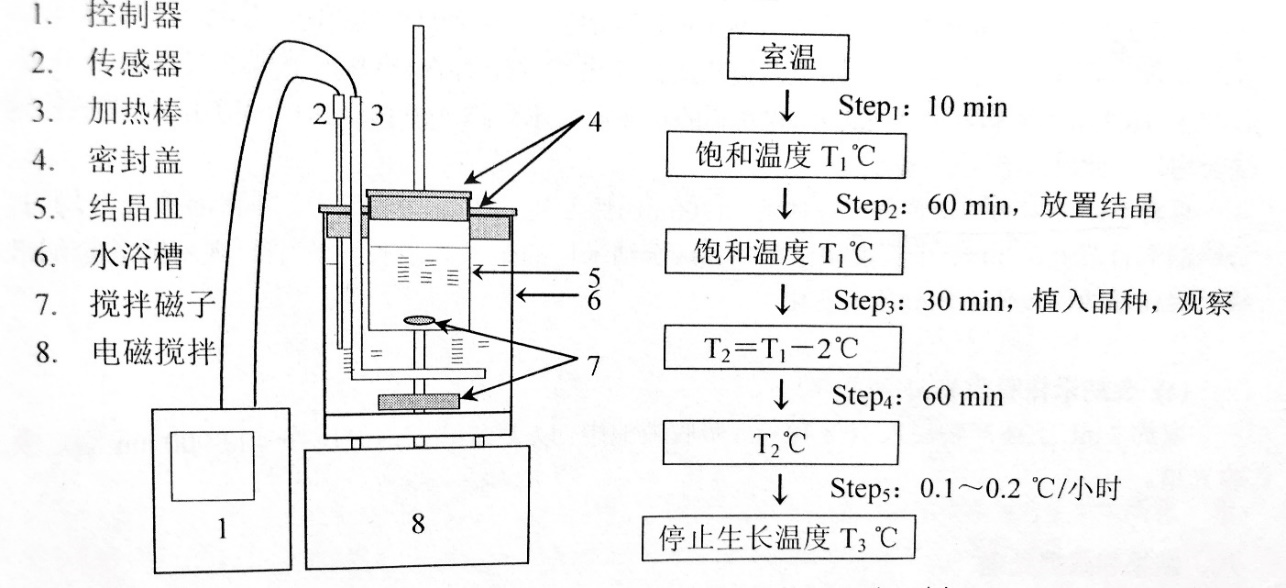
\includegraphics[scale=1.0]{jiangwenshebei.png}
        \caption{控温设备图示}
        \label{jiangwenshebei}
    \end{figure}
    \paragraph{(2)配置KDP饱和溶液}
    在烧杯中加入120ml(实际120.18g)去离子水,加入$43\celsius$温度下饱和溶液含量的KDP,理论为43.8g
    (实际称取43.84g)。在$\approx 80\celsius$的水浴中加热溶解,用砂芯漏斗将溶液趁热过滤
    入结晶皿中,将结晶皿继续置于水浴中加热15min-20min。然后将结晶皿放入加热装置中,开启加热程序。
    \paragraph{(3)植入晶种}
    在step2中将一块扁平略长的没有明显缺陷的晶种用棉线系好,先悬挂在溶液上方短暂预热,然后悬挂于溶液表面
    大约1cm处。晶种的质量为:0.43g。
    \paragraph{(4)取出晶体}
    同周周日15:00去实验室取出晶体,此时观察到烧杯底部已经析出了少量晶体。
    可以观察到晶体上方与棉线的接触点附近长出了一颗小的晶体、棉线与溶液表面的接触点、
    也有多晶析出但是并没有触及本体。可以从图中看出晶体表面没有任何缺陷,
    生长比较完美,基本按照图\ref{KDP crystal grow}所示的晶面生长,
    内部可以看到隐约的与晶种的接触面。最终的晶体质量为2.03g,
    并没有长得很大。
    \begin{figure}[htbp]
        \centering 
        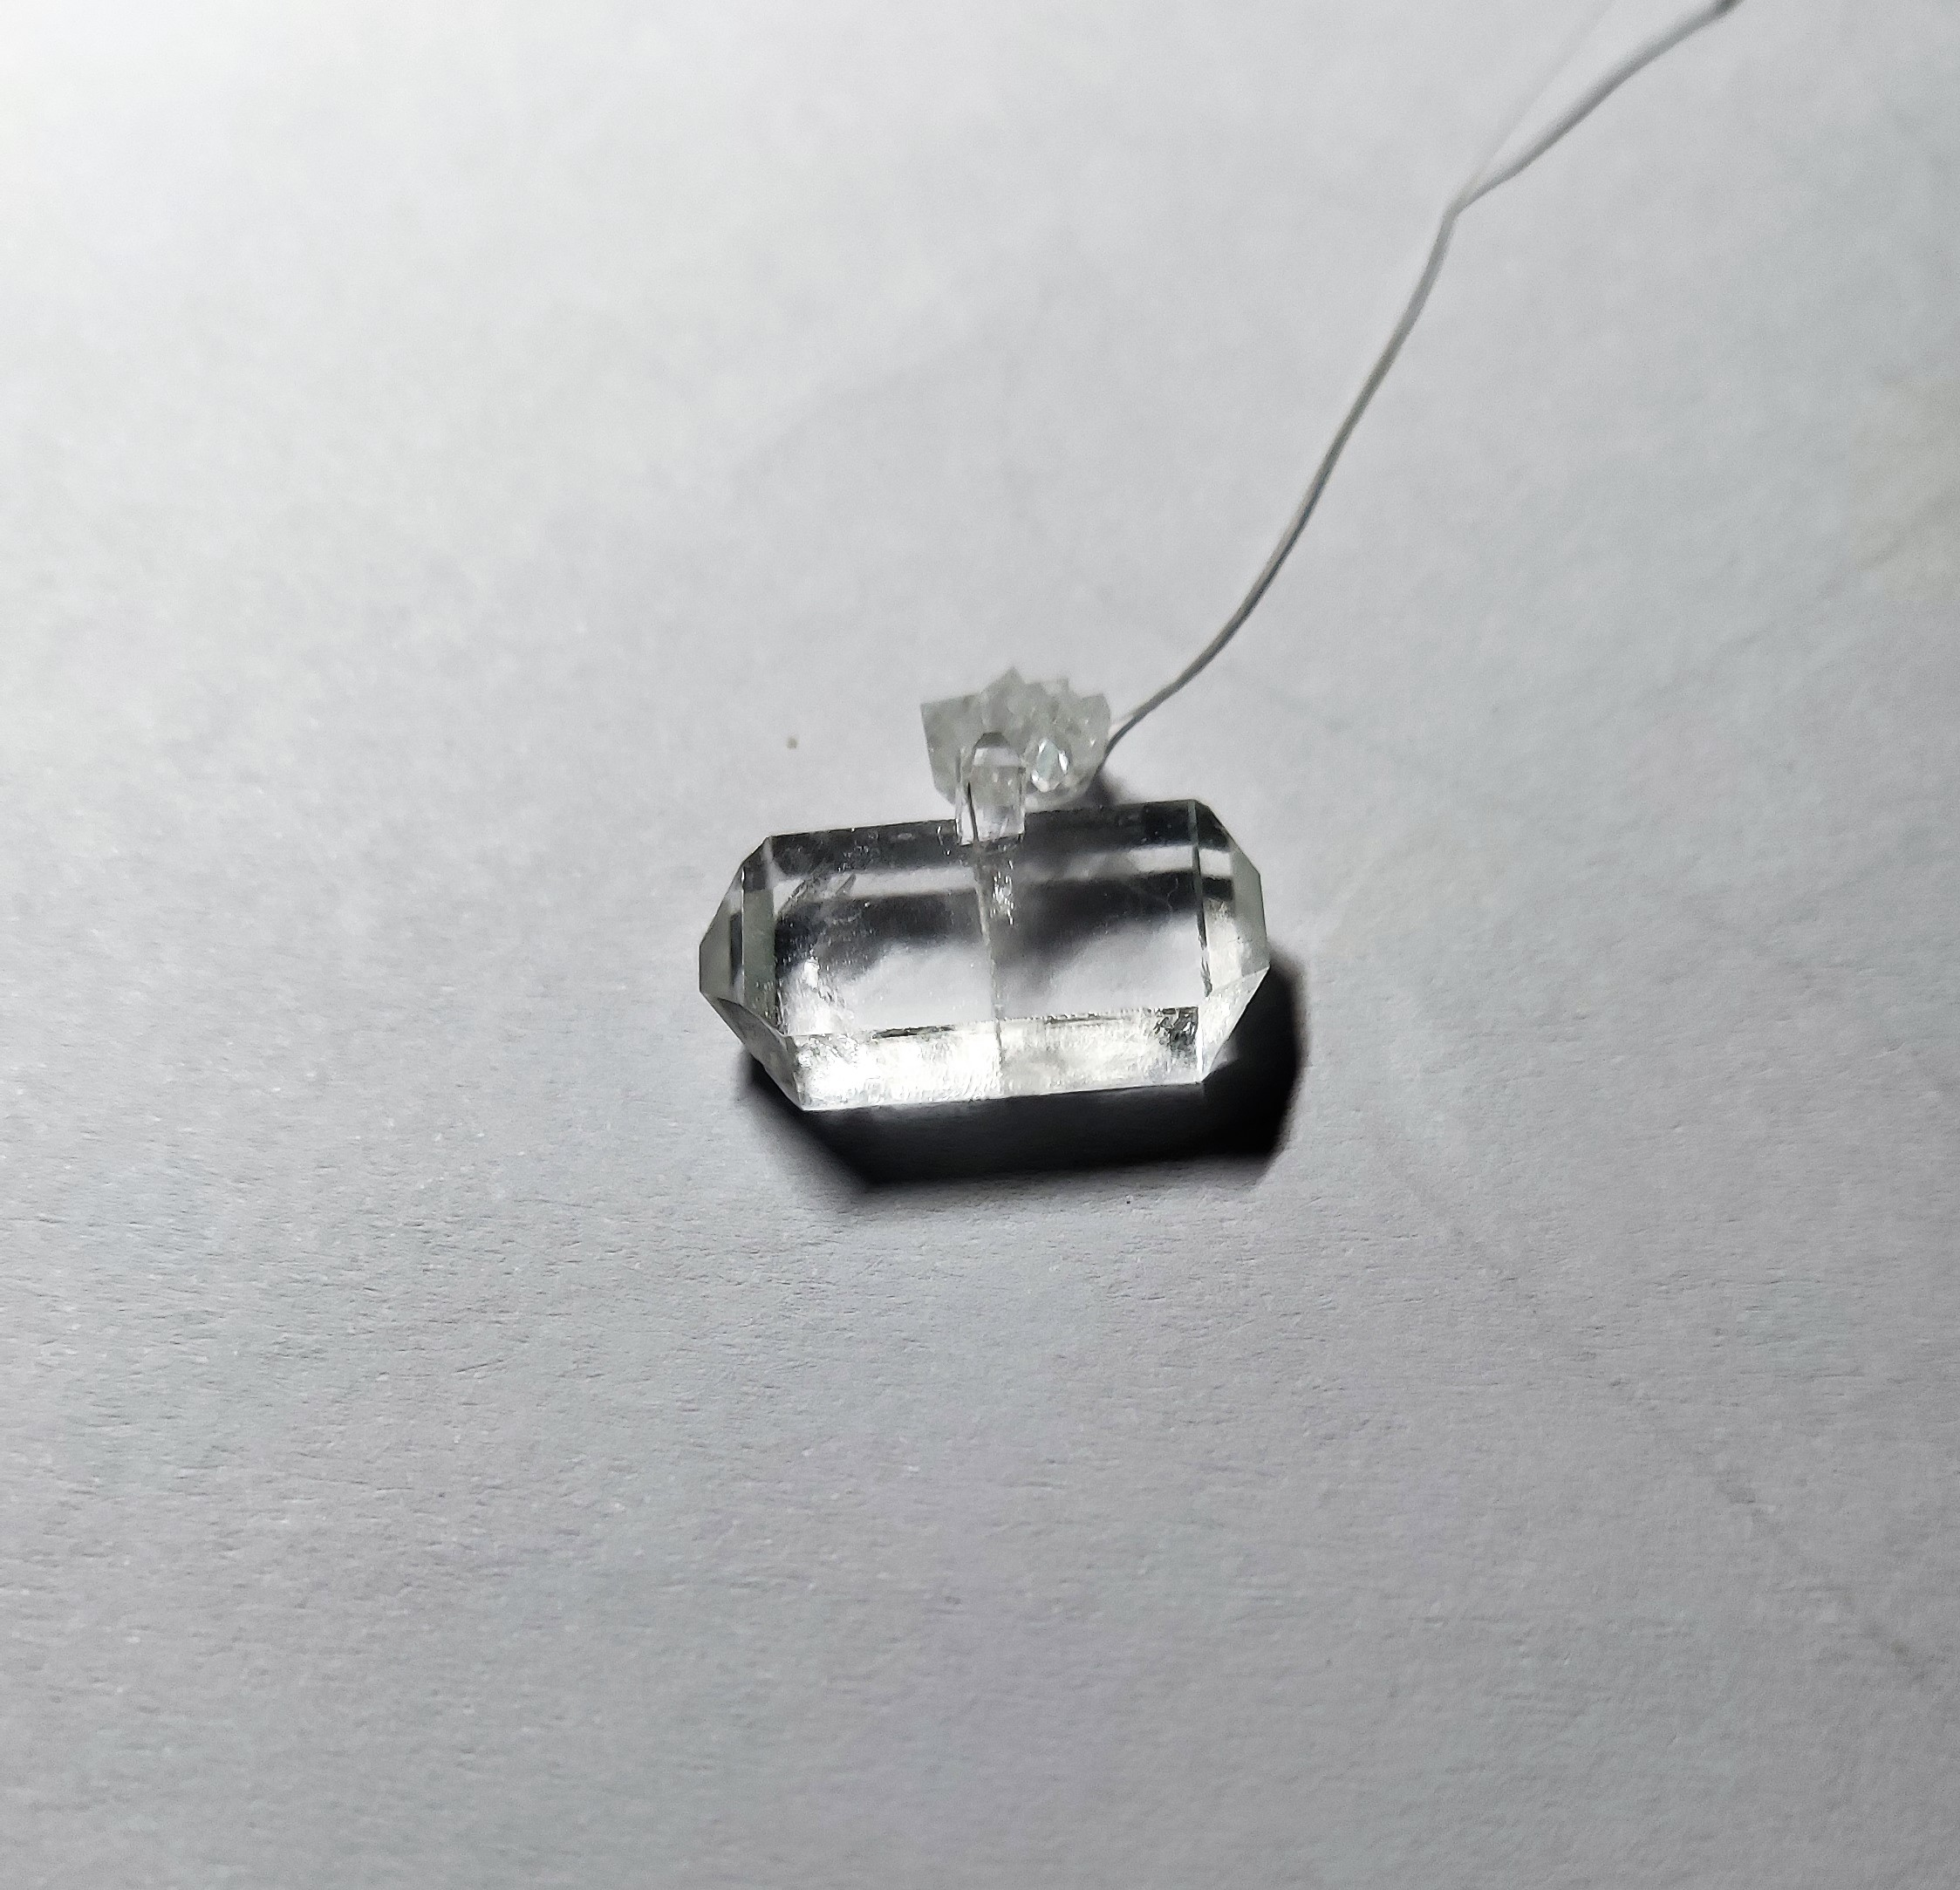
\includegraphics[scale=0.11]{mycrystal.jpg}
        \caption{实验者本人培养的晶体}
        \label{my crystal}
    \end{figure}
    \subsection{金纳米棒的制备}
    \paragraph{(1)配制CTAB水溶液}
    称取1.34g CTAB(Mr=364.45g/mol)加入到80.02g去离子水中,水浴加热溶解,得到0.05mol/L
    的CTAB溶液。
    \paragraph{(2)金种子的制备}
    实验室老师已经制备好了。
    \paragraph{(3)金纳米棒的制备}
    用移液枪取\ce{HAuCl_4}水溶液1ml(0.01mol/L)于离心管中,快速加入到20ml CTAB溶液中混匀,
    此时溶液呈现出橙黄色。再依次加入\ce{AgNO_3}水溶液$30\mu$L(重复这个实验,将硝酸银溶液
    的量改为50$\mu$L,100$\mu$L,150$\mu$L)、400$\mu$L, 1.0mol/L的盐酸、160$\mu$L, 0.1mol/L
    的新制维生素C溶液,溶液混匀后颜色从橙黄色变为无色,说明三价金被还原为一价金(溶液没有
    浑浊也没有沉淀生成,说明不可能是析出了单质金)。将200$\mu$L纳米金种子溶液加入其中,
    放置于30$\celsius$的恒温水浴槽中完成纳米金棒的生长,胶体溶液从最开始的几乎无色透明,颜色逐渐
    加深,加入$30\mu$L硝酸银的离心管从无色逐渐变为浅紫红色,颜色渐渐加深;加入$50\mu$L硝酸银
    的离心管从无色变为浅紫色,逐渐加深为深蓝紫色;加入 $100\mu$L硝酸银的离心管从无色逐渐
    变为褐紫色;加入$150\mu$L硝酸银的离心管溶液从无色逐渐变为深红褐色。
    最终的效果参见图\ref{Au nano bar}
    \begin{figure}[htbp]
        \centering
        \includegraphics[scale=0.1]{Aubar.jpg}
        \caption{金纳米棒溶液}
        \label{Au nano bar}
    \end{figure}
    \paragraph{(4)金纳米棒的吸收光谱测试}
    取少量产物溶液加入比色皿(加满多半比色皿,注意加入$100\mu$L与$150\mu$L硝酸银
    的产物溶液要用去离子水稀释),测定其在400-100nm的吸收光谱。
    吸收光谱结果参见图 ,其上已经标注了对应加入的硝酸银的量。
    \begin{figure}
        \centering
        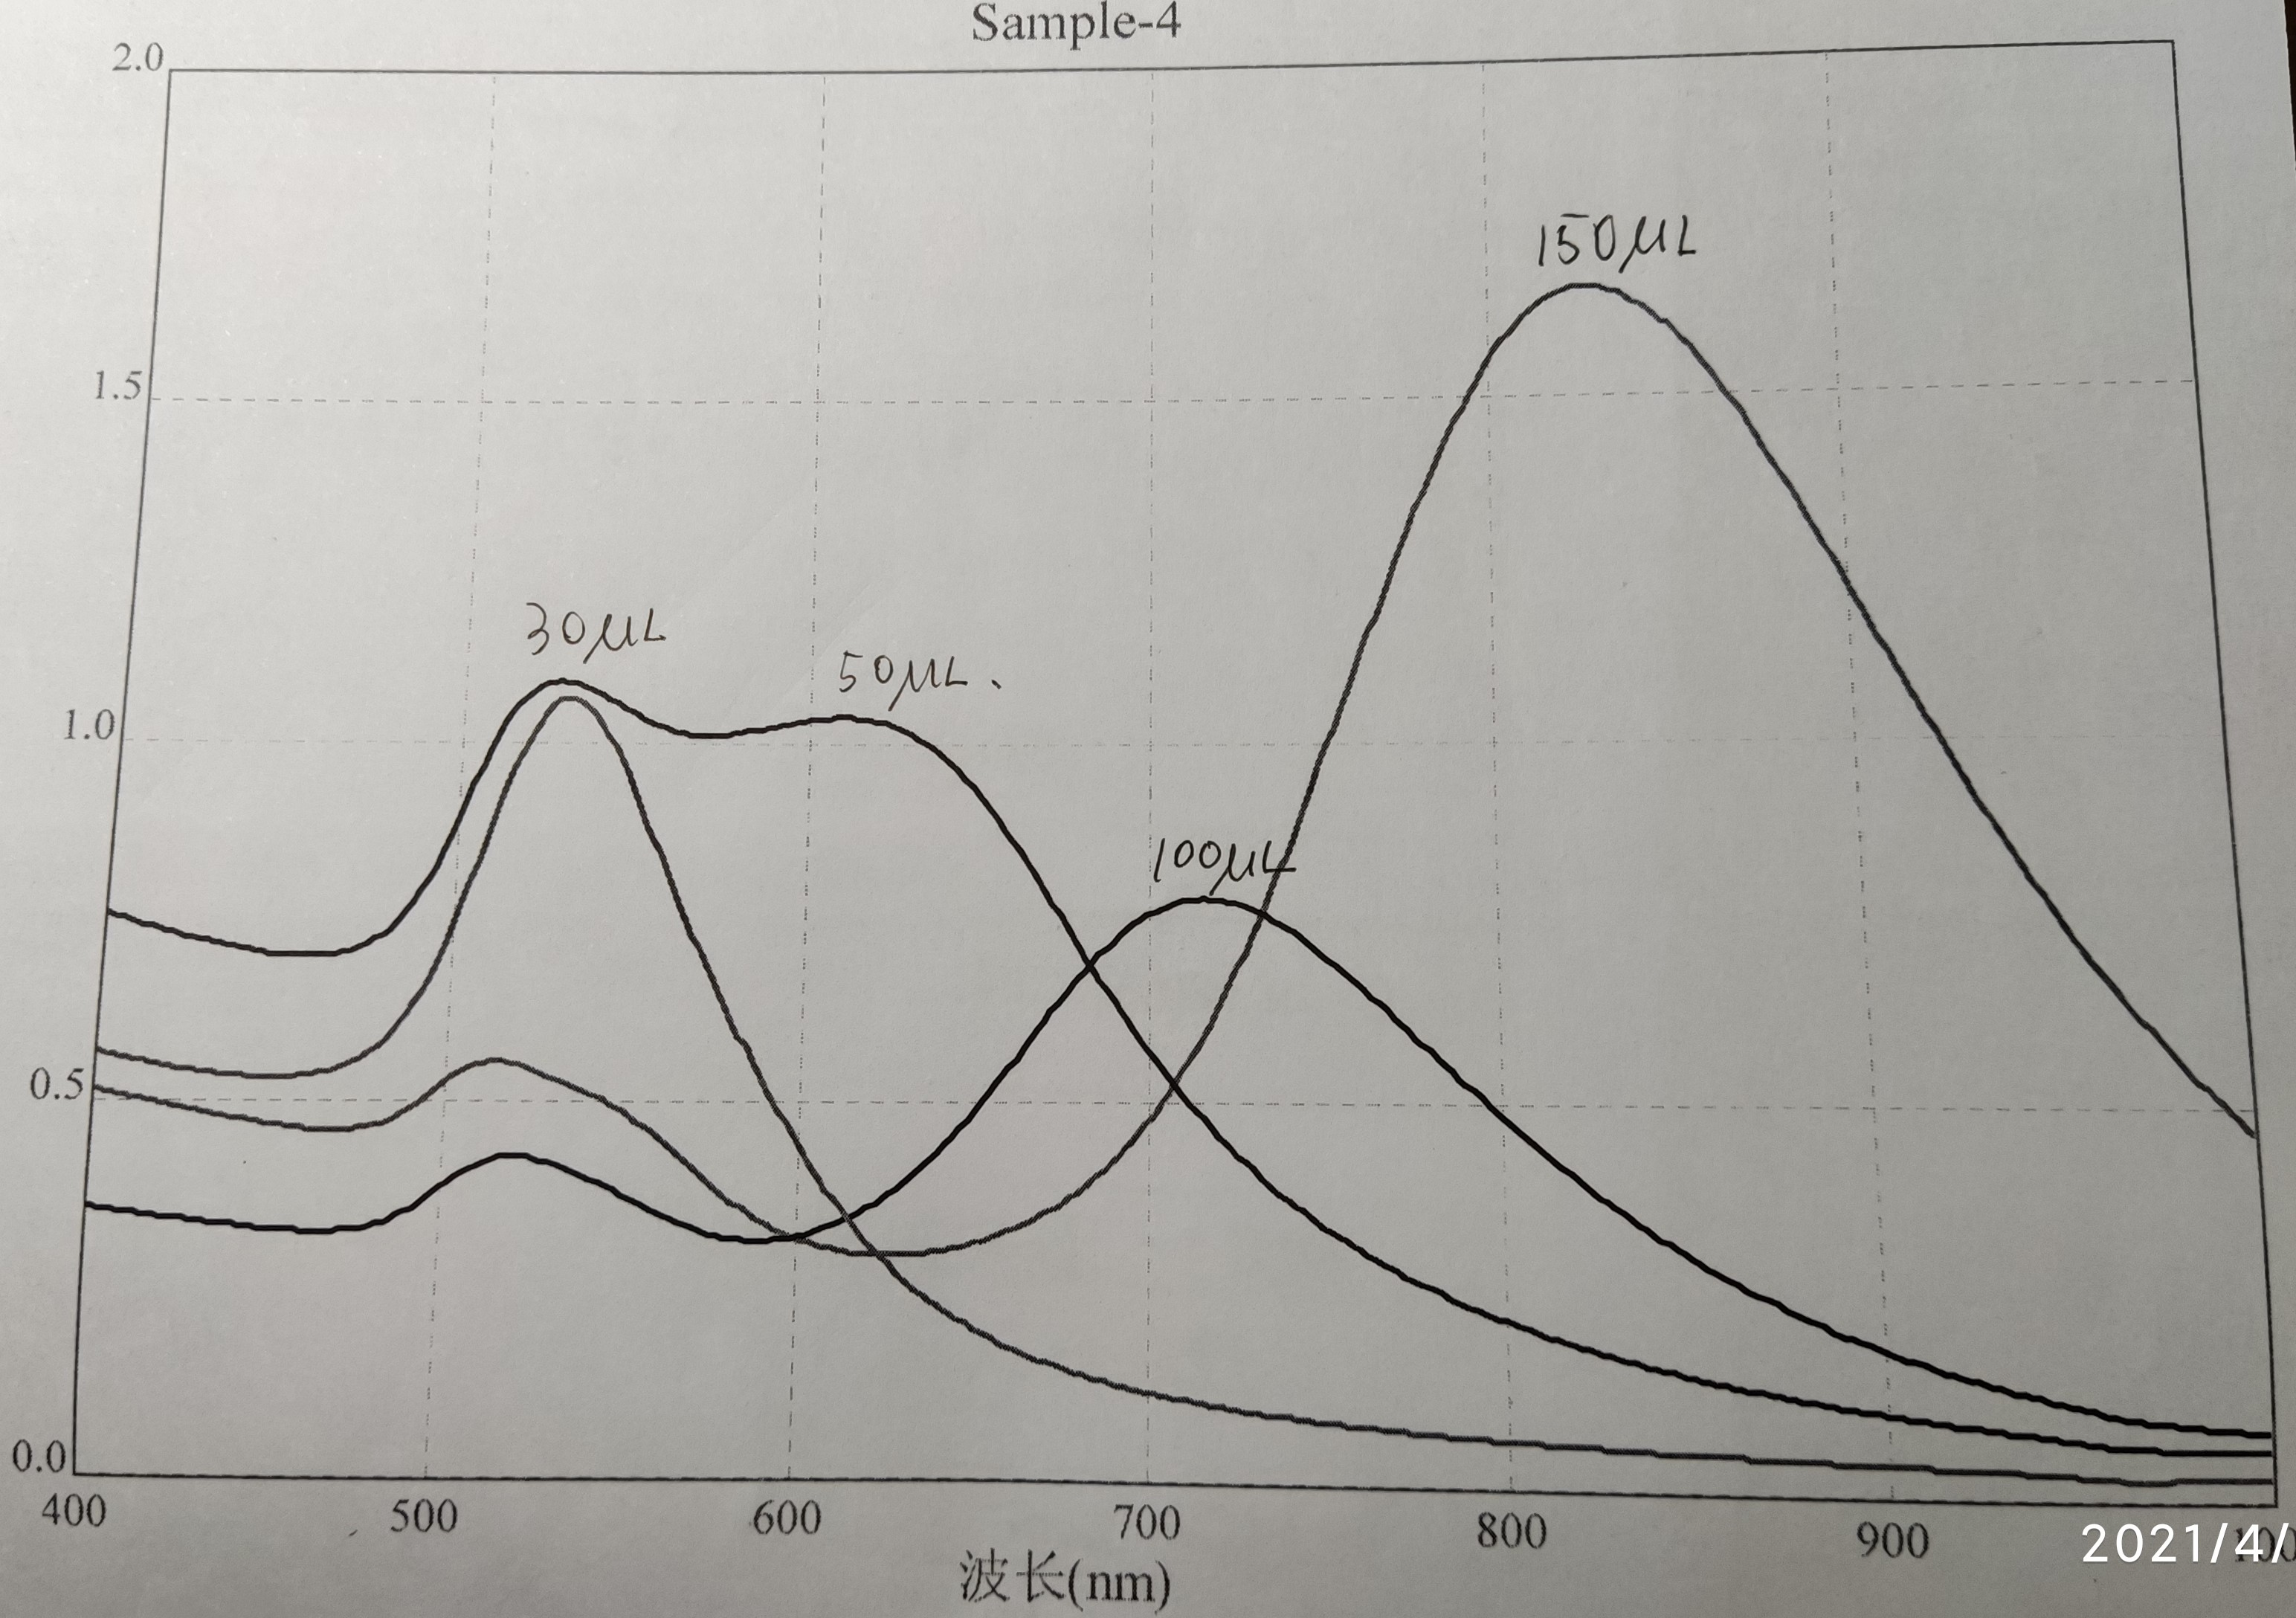
\includegraphics[scale=0.1]{spectrum.jpg}
        \caption{金纳米棒光谱}
        \label{spectrum of Au nano}
    \end{figure}
    \section{结果与讨论}
    \subsection{单晶生长}
    可以根据前面的讨论计算出晶体生长了1.60g,由于取出晶体时距离降温结束还有大概24h,因此
    可以推算出取出晶体时溶液的温度为38.5$\celsius$,可以根据实验教材给出的近似公式计算出
    溶解度为33.74g/100g,因此溶液中残余40.49g,理论上晶体生长量为:3.31g,实际生长量
    约为理论生长量的一半。生长量偏小的原因是结晶皿底部有少量晶体析出(实验室中有一位同学
    结晶皿底部没有析出晶体),这说明了溶液中
    残存有少量机械杂质充当了晶核,提示我们以后生长晶体一定要保持溶液与结晶皿的洁净。
    取晶体时仔细观察了同学的晶体,基本上都出现了棉线穿过晶体表面的地方生长多晶的现象,
    这有可能是悬挂法长单晶的一个固有缺陷。
    \subsection{金纳米棒的生长}
    实验中探究了加入不同量的硝酸银对于金纳米棒生长的影响。可以看出,当加入$30\mu$L硝酸银
    时,溶液的只有一个在520nm左右的吸收峰,对应了溶液看起来为紫红色,
    这是球状纳米金颗粒的吸收;当加入$50\mu$L硝酸银时,吸收曲线出现了明显的变化,
    在520nm峰的右侧620nm左右出现了新的吸收峰,这说明纳米金颗粒已经不再是球对称的,开始
    展现出各向异性;当加入$100\mu$L硝酸银时,可以观察到溶液在710nm处有一个明显的吸收峰,
    而520nm处的吸收峰基本上没有变动;当加入$150\mu$L硝酸银时,溶液第二个吸收峰继续红移到
    830nm处,第一个吸收峰的位置依然没有明显变化。那么可以看出,随着硝酸银的用量增加,
    短波处的吸收峰没有变化,长波处的吸收峰逐渐红移,这说明随着硝酸银用量的增加,金纳米棒的直径
    没有明显的变化,而长度不断增长,从而导致了纵向振动的频率下降,进一步导致吸收光的频率下降。

    \bibliographystyle{plain}
	\bibliography{ref}
\end{document}